%%%%%%%%%%%%%%%%%%%%%%%%%%%%%%%%%%%%%%%%%%%%%%
% To select a journal, use its code for the 
% journal= option in the \documentclass command.
% The journal codes for this template are:
% 
% Journal of Law and Courts: jlc
% Macroeconomic Dynamics: mdy
% State Politics & Policy Quarterly: spq
%%%%%%%%%%%%%%%%%%%%%%%%%%%%%%%%%%%%%%%%%%%%%%
\documentclass[
  journal=small,
  manuscript=ARTICULO-CIENTIFICO,  % Use a - if you need a space e.g. "research-article"
  year=2025
]{cup-journal}

\usepackage{forest}
\usepackage{amsmath}
\usepackage[nopatch]{microtype}
\usepackage{booktabs}

\title{Procesos en Linux}

\author{Merino Vidal Mateo Alejandro}
\affiliation{Universidad Mayor de San Simón \\ 
\texttt{Cochabamba, Bolivia }\\  
\texttt{202301308@est.umss.edu}}

\keywords{proceso, jerarquía, sistema operativo} 

\begin{document}

\begin{abstract}
El presente informe tiene como objetivo ejecutar dos códigos en lenguaje C, relacionados con la creación e identificación de procesos. Para ello, se utilizó una distribución de Linux denominada "adios". Sin embargo, dado que el sistema operativo principal es Windows, fue necesario recurrir a una máquina virtual, específicamente VirtualBox, que permitió ejecutar dicha distribución dentro de un entorno virtualizado.
\end{abstract}

\section{Introducción}
Cada acción iniciada, desde abrir el shell de explorer hasta ejecutar un simple comando conlleva diversos procesos.
Estos procesos están basados en una jerarquía, similar al de un árbol genealógico, por lo que es necesario emplear  términos como padres e hijos para observar el nivel y relación de cada uno.
\\
\\
Cada proceso cuenta con su propia información, incluyendo su identificador de proceso (PID) y el identificador de su proceso padre (PPID).
Un proceso padre es aquel que crea uno o varios procesos hijos a través de una llamada al sistema.
\\
\\
Los procesos hijos heredan casi todo del padre como: código, variables, archivos abiertos, etc. 
Cada uno cuenta con su propio identificador único de proceso, distinto al del padre.\\ 
Además, tienen la capacidad de ejecutarse en paralelo con el padre o esperar instrucciones, dependiendo de la situación.
\\
\\
Es posible realizar esa creación de procesos mediante la llamada al sistema fork().
\\
\\
\fbox{
    \begin{minipage}{0.9\textwidth}
        \textbf{Fork: Es una llamada al sistema en Unix/Linux, que permite a un proceso crear una copia de sí mismo, generando un nuevo proceso hijo. Este proceso hijo hereda la mayoría de las características del proceso padre, pero tendrá un identificador de proceso único.
        Tanto el proceso padre como el hijo continuarán ejecutándose desde el mismo punto después del fork().
}
    \end{minipage}
}
\\
\\
 Esta llamada al sistema también posee un valor de retorno, el cual brinda información importante, es decir, si el valor de retorno es:
        \begin{itemize}
        \item Numero Positivo: Estamos en el proceso padre y devuelve el PID del proceso hijo creado.
        \\
        \item Cero: Estamos en el proceso hijo.
        \\
        \item Menos Uno: Hubo un error y no se creo el proceso hijo.
\end{itemize}  
\section{Desarrollo}
\vspace{0.9em}
\subsection{Procedimiento}
\vspace{0.6em}
Para el presente trabajo, se tuvieron que seguir una serie de instrucciones, las cuales permitieron utilizar la distribucion "adios" de linux y ejecutar los códigos necesarios.
\\
\\
Entre esas instrucciones están:
\begin{enumerate}
    
    \item Copiar y pegar los dos códigos correspondientes de la practica de TSO a archivos de texto (txt); y almacenarlos en un USB. 
    \begin{figure}[h]
    \centering
    \includegraphics[width=0.95\textwidth]{Codigo1TXT.png}
    \caption{Codigo1}
    \label{1}
    \end{figure} \\
    
    Se observa en la fig.\ref{1} una implementación en C, la cual permite la obtención del identificador del proceso mediante la llamada al sistema (system call).\\
    Se obtiene como resultado el identificador del proceso padre e hijo.
    \\
    \\
    \\
    \\
    \\
    \\
    \\
    \begin{figure}[h]
    \centering
    \includegraphics[width=0.95\textwidth]{Codigo2TXT.png}
    \caption{Codigo2}
    \label{2}
    \end{figure} \\
     Se observa en la fig.\ref{2} una implementación en C, la cual permite la creación de un proceso hijo a través del system call "fork()", el cual sera una copia del proceso en el que estamos actualmente, que seria el padre.
    \\
    \\
    Se obtiene como resultado:
    \\
    \\
    -El PID del proceso padre y el PID de su padre (el shell).
    \\
    -El PID del proceso hijo y el PID del proceso padre (que es el proceso original antes de ejecutar fork() ).
    \\
    \\
    \item Iniciar la herramienta "Virtual Box", la cual permitirá ejecutar la distribucion "adios" de linux en una maquina virtual.
    \begin{figure}[h]
    \centering
    \includegraphics[width=0.95\textwidth]{VirtualBox.png}
    \caption{Virtual Box}
    \label{fig:etiqueta}
    \end{figure}
    \\
    \\
    \\
    \\
    \\
    \item Ejecutar el emulador con la distribucion de linux, conocida como "adios".
    \begin{figure}[h]
    \centering
    \includegraphics[width=0.95\linewidth]{Emulador.png}
    \caption{Emulador}
    \label{3}
    \end{figure}
    \\
    Se observa en la fig.\ref{3} el entorno de trabajo proporcionado por la maquina virtual, así como un acceso directo al directorio ESD-USB, que confirma el reconocimiento del USB y la presencia de los archivos TXT con los códigos a ejecutar.
    \\
    \item Se inicializa el CMD o la interfaz de comandos del sistema. 
    \begin{figure}[h]
    \centering
    \includegraphics[width=0.95\linewidth]{IngresoDirectorioUSB.png}
    \caption{Ingreso al directorio del USB}
    \label{4}
    \end{figure}
    \\
    \\
    \\
    \\
    \\
    \\
    Se observa en la fig.\ref{4} que mediante los comandos "ls" y "ls -l", se obtiene un listado de los directorios y archivos contenidos en el directorio actual. \\
    Posteriormente, se retrocede varios directorios mediante el comando "cd ..", hasta llegar al directorio raíz que contiene el directorio "media".
    Se accede al directorio "media" que contiene el directorio "ESD-USB" correspondiente al USB y se accede a ese directorio.
     \\
     \\
    \item Una vez ubicados en el directorio ESD-USB, se pide un listado de los archivos, para confirmar la existencia de cada código con su correspondiente archivo TXT.
    \begin{figure}[h]
    \centering
    \includegraphics[width=0.95\linewidth]{ListadoArchivos.png}
    \caption{Lista de archivos en el directorio ESD-USB}
    \label{5}
    \end{figure}
    \\
    \\
    \\
    \\
    \\
    \\
    \\
    \\
    \\
    \\
    \\
    \\
    \\
    \\
    \\
    \\
    \\
    Se observa en la fig.\ref{5} la existencia de los dos archivos TXT, que están con el nombre de "TSO\_Codigo1.txt" y "TSO\_Codigo2.txt".
    \\
    \item Se utiliza el comando "mv" para cambiar el nombre de los archivos y sus extensiones de txt a c.
    Este cambio se realiza para ambos archivos txt con la finalidad de poder compilarlos y ejecutarlos después.
    \begin{figure}[h]
    \centering
    \includegraphics[width=0.95\linewidth]{Renombrando.png}
    \caption{Renombrado de los archivos TXT}
    \label{6}
    \end{figure}
    \\
    Se observa en la fig.\ref{6} que el archivo "TSO\_Codigo1.txt" cambio a "TSO\_Codigo1C.c" y el archivo "TSO\_Codigo2.txt" cambio a "TSO\_Codigo2C.c".
    \\
    \\
     \item Se utiliza el comando "cat" para observar el contenido de ambos archivos, en los cuales se puede detectar errores de sintaxis como el uso de `;' en los \#include de ambos archivos y la diferencia de comillas dobles a las aceptadas.
    \\
    \\
    \\
    \begin{figure}[h]
    \centering
    \includegraphics[width=0.85\linewidth]{VisualizacionCodigo1.png}
    \caption{Contenido del archivo TSO\_Codigo1C.c}
    \label{fig:etiqueta}
    \end{figure}
    \begin{figure}[h]
    \centering
    \includegraphics[width=0.85\linewidth]{VisualizacionCodigo2.png}
    \caption{Contenido del archivo TSO\_Codigo2C.c}
    \label{fig:etiqueta}
    \end{figure}
    \hfill \break
    \hfill \break
    \hfill \break
    \item Se utiliza el comando "nano" para editar el código en ambos archivos y eliminar la presencia de ';' en cada \#include, como también reemplazar las comillas dobles no aceptadas por las correctas.
    \begin{figure}[h]
    \centering
    \includegraphics[width=0.93\linewidth]{ActivarNano.png}
    \caption{Uso del comando "nano"}
    \label{fig:etiqueta}
    \end{figure}
    \begin{figure}[h]
    \centering
    \includegraphics[width=0.95\linewidth]{Correccion1.png}
    \caption{Corrección del archivo TSO\_Codigo1C.c}
    \label{fig:etiqueta}
    \end{figure}
    \begin{figure}[h]
    \centering
    \includegraphics[width=0.95\linewidth]{Correccion2.png}
    \caption{Corrección del archivo TSO\_Codigo2C.c}
    \label{fig:etiqueta}
    \end{figure}
    \\
    \\
    \\
    \\
    \\
    \\
    \\
    \item Se utiliza el comando "gcc -o" para compilar ambos archivos con la extensión c.
    Al hacer esto, se crea un nuevo archivo que es un ejecutable, por cada uno. \\
    Del archivo "TSO\_Codigo1C.c" se crea el ejecutable "compilado1" y del archivo "TSO\_Codigo2C.c" se crea el ejecutable "compilado2".

    \begin{figure}[h]
    \centering
    \includegraphics[width=0.95\linewidth]{CompiladoArchivos.png}
    \caption{Uso del comando "gcc -o"}
    \label{fig:etiqueta}
    \end{figure}

    \begin{figure}[h]
    \centering
    \includegraphics[width=0.95\linewidth]{ListadoArchivosCompilados.png}
    \caption{Verificación de archivos compilados}
    \label{14}
    \end{figure}
    \hfill \break
    \hfill \break
    \hfill \break
    \hfill \break
    \hfill \break
    \hfill \break
    \hfill \break
    \hfill \break
    Se observa en la fig.\ref{14} , que mediante el comando "ls" es posibles confirmar la existencia de los nuevos archivos compilados, nombrados como "compilado1" y "compilado2".
    \\
    \\
    \item Se utiliza el comando "./" para ejecutar los archivos compilados "compilado1" y "compilado2".
    \\
    \\
    En el caso del archivo "compilado1", este nos da como resultado:
    \begin{center}
    \fbox{
    \begin{minipage}{0.9\textwidth}
    \texttt{[adios@localhost ESD-USB] \$ ./compilado1} \\
    \texttt{Identificador de proceso: 2487} \\
    \texttt{Identificador del proceso padre: 2376}
    \end{minipage}
    }
    \end{center}
    
    En el caso del archivo "compilado2", este nos da como resultado:
    \begin{center}
    \fbox{
    \begin{minipage}{0.9\textwidth}
    \texttt{[adios@localhost ESD-USB] \$ ./compilado2} \\
    \texttt{Proceso 2502; padre = 2501} \\
    \texttt{Proceso 2501; padre = 2376}
    \end{minipage}
    }
    \end{center}

    Posteriormente, al ejecutar los archivos varias veces, nos permite tener mayor información sobre los identificadores de los procesos.
    \\
    \\
    \\
     \begin{figure}[h]
    \centering
    \includegraphics[width=0.7\linewidth]{Ejecucion1.png}
    \caption{Ejecución del archivo "compilado1"}
    \label{15}
    \end{figure}
    \\
    Se observa en la fig.\ref{15} que el proceso padre, que es el shell en el que estamos tiene como identificador 2376 y posee diversos hijos con distintos identificadores cada uno.
    Esto da como resultado una estructura similar a:
    \\
    \\
    
    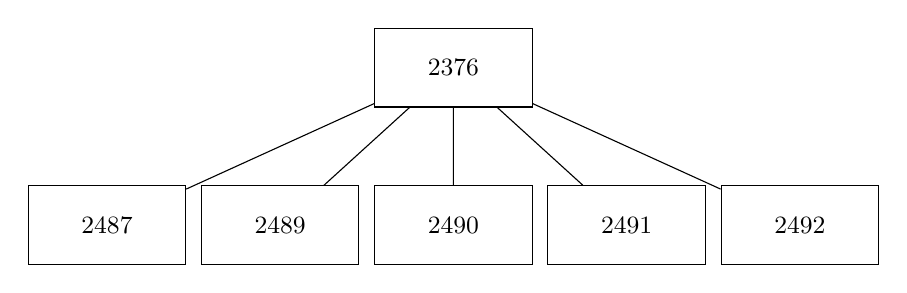
\begin{tikzpicture}[
      level 1/.style={sibling distance=2.2cm, level distance=2cm}, % Ajustamos distancias
      level 2/.style={sibling distance=2cm},
      process/.style={draw, rectangle, minimum width=2cm, minimum height=1cm, text centered, font=\small} % Reducir el ancho de los bloques
    ]
    % Root process
    \node [process] {2376}
      % Child processes of 2376
      child {node [process] {2487}}
      child {node [process] {2489}}
      child {node [process] {2490}}
      child {node [process] {2491}}
      child {node [process] {2492}};
    \end{tikzpicture}
    \hfill \break
     \begin{figure}[h]
    \centering
    \includegraphics[width=0.7\linewidth]{Ejecucion2.png}
    \caption{Ejecución del archivo "compilado2"}
    \label{16}
    \end{figure}
    \hfill \break
    \hfill \break
    \hfill \break
    \hfill \break
    \hfill \break
    \hfill \break
    \hfill \break
    \hfill \break
    \hfill \break
    \hfill \break
    \hfill \break
    \hfill \break
    \hfill \break
    \hfill \break
    \hfill \break
    Se observa en la fig.\ref{16} que el proceso padre, que es el shell en el que estamos, tiene como identificador 2376 y posee diversos hijos con distintos identificadores. Como consecuencia de ejecutar el programa múltiples veces, se muestra que el proceso 2376 es el padre de los procesos 2501, 2503, 2505, 2507, y 2509. Estos, a su vez, crean sus propios hijos, como los procesos 2502, 2504, 2506, 2508, y 2510. \\
    Esto da como resultado una estructura similar a: 
    \hfill \break
    \hfill \break
   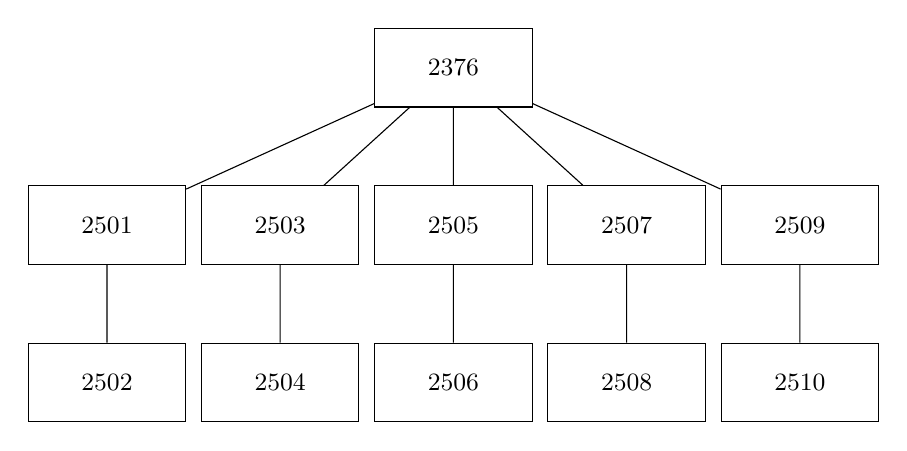
\begin{tikzpicture}[
      level 1/.style={sibling distance=2.2cm, level distance=2cm}, % Reducir la distancia entre nodos
      level 2/.style={sibling distance=2cm},
      process/.style={draw, rectangle, minimum width=2cm, minimum height=1cm, text centered, font=\small} % Reducir el ancho de los cuadros
    ]
    % Root process
    \node [process] {2376}
      % Child processes of 2376
      child {node [process] {2501}
        child {node [process] {2502}} % Child of 2501
      }
      child {node [process] {2503}
        child {node [process] {2504}} % Child of 2503
      }
      child {node [process] {2505}
        child {node [process] {2506}} % Child of 2505
      }
      child {node [process] {2507}
        child {node [process] {2508}} % Child of 2507
      }
      child {node [process] {2509}
        child {node [process] {2510}} % Child of 2509
      };
    \end{tikzpicture}
    
    \end{enumerate}
\hfill \break
\hfill \break
\hfill \break
\hfill \break
\hfill \break
\subsection{Cuestionario}
\hfill \break
1) ¿El proceso hijo empieza la ejecución del código en su punto de inicio, o en la sentencia que está después del fork()?
\\
\\
R.-Empieza en la sentencia después del fork(), ya que el proceso hijo se crea en el momento que se llama a fork(). Es a partir de ese punto que el proceso hijo adquiere un identificador único y las mismas características que el proceso padre. Ambos procesos, continúan ejecutando el código a partir de la sentencia que sigue al fork(), pero de forma independiente.
\\
\\
2) Observar, que el hijo no es totalmente idéntico al padre, algunos de los valores del
BCP han de ser distintos. Responder: ¿cuáles deberían ser las diferencias más
importantes?

\begin{table}[ht]
\centering
\begin{tabular}{|p{8cm}|c|}
\hline
\textbf{Afirmación} & \textbf{Verdadero (V) / Falso (F)} \\
\hline
El proceso hijo tiene su propio identificador de proceso, distinto al del padre. & V \\
\hline
El proceso hijo tiene una nueva descripción de la memoria. Aunque el hijo tenga los mismos segmentos con el mismo contenido, no tienen por qué estar en la misma zona de memoria. & V \\
\hline
El tiempo de ejecución del proceso hijo se iguala a cero. & V \\
\hline
Todas las alarmas pendientes se desactivan en el proceso hijo. & V \\
\hline
El conjunto de señales pendientes se pone a vacío. & V \\
\hline
El valor que retorna el sistema operativo como resultado del fork es distinto en el hijo y el padre. & V \\
\hline
\end{tabular}
\end{table}
\hfill \break
3) Observar que las modificaciones que realice el proceso padre sobre sus registros e
imagen de memoria después del fork() no afectan al hijo y, viceversa, las del hijo no
afectan al padre. Sin embargo, el proceso hijo tiene su propia copia de los
descriptores del proceso padre.
Este hace que el hijo tenga acceso a los archivos abiertos por el proceso padre. El
padre y el hijo comparten el puntero de posición de los archivos abiertos en el padre.
Responder si esto podría afectar y de que manera a lo que acaba de observar.
\\
\\
R.-Se observó durante la ejecución del código, que el proceso hijo en realidad tiene una copia independiente de los registros e información del proceso padre. Sin embargo, este también posee los descriptores o referencias de archivos a los que apunta el proceso padre, por lo que, si el padre realiza una operación de lectura o escritura sobre un archivo, este llega a afectar a la posición del puntero de archivo del hijo, ya que ambos lo comparten.
\\
\\
\\
\\
\section{Conclusión}
\begin{itemize}
  \item El uso de la llamada al sistema fork() permite crear procesos hijos que heredan características del proceso padre. Sin embargo, cada hijo cuenta con su propio identificador, distinto al del padre.
  \\
  \item La jerarquía de procesos, con un proceso padre que genera procesos hijos, es clave para comprender cómo se organiza y gestiona el flujo de ejecución en un sistema. Esta organización de los procesos es similar al de un árbol genealógico, por lo que es posible representarla gráficamente para una mejor comprensión.
  \\
  \item La ejecución de programas en la distribución Linux "adios", mediante la aplicación "VirtualBox" que se uso para la visualización, resalta la importancia de entender los comandos básicos del sistema operativo y la gestión de procesos. 
  
\end{itemize}

\end{document}